% Use only LaTeX2e, calling the article.cls class and 12-point type.

\documentclass[12pt]{article}

% Users of the {thebibliography} environment or BibTeX should use the
% scicite.sty package, downloadable from *Science* at
% http://www.sciencemag.org/authors/preparing-manuscripts-using-latex 
% This package should properly format in-text
% reference calls and reference-list numbers.

\usepackage{scicite}
\usepackage{xspace}

\usepackage{times}
\usepackage{graphicx}


% The preamble here sets up a lot of new/revised commands and
% environments.  It's annoying, but please do *not* try to strip these
% out into a separate .sty file (which could lead to the loss of some
% information when we convert the file to other formats).  Instead, keep
% them in the preamble of your main LaTeX source file.


% The following parameters seem to provide a reasonable page setup.

\topmargin 0.0cm
\oddsidemargin 0.2cm
\textwidth 16cm 
\textheight 21cm
\footskip 1.0cm


%The next command sets up an environment for the abstract to your paper.

\newenvironment{sciabstract}{%
\begin{quote} \bf  }
{\end{quote}}

\usepackage{xcolor}
\newcommand{\bam}[1]{\textcolor{green!65!black}{\textbf{[BAM: #1]}}}


\date{}



\newcommand{\nraojansky}{\footnotesize{\it{Jansky fellow of the National Radio Astronomy Observatory, 1003 Lopezville Rd, Socorro, NM 87801 USA }}}
\newcommand{\nrao}{\footnotesize{\it{National Radio Astronomy Observatory, 1003 Lopezville Rd, Socorro, NM 87801 USA }}}
\newcommand{\nraocv}{\footnotesize{\it{National Radio Astronomy Observatory, Charlottesville, VA 22903 USA }}}
\newcommand{\cfa}{\footnotesize{\it{Harvard-Smithsonian Center for Astrophysics, Cambridge, MA 02138 USA }}}
\newcommand{\hubble}{\footnotesize{B.A.M. is a Hubble Fellow of the National Radio Astronomy Observatory.}}


\newcommand{\radboud}{\footnotesize{\it{Department of Astrophysics/IMAPP, Radboud University Nijmegen, PO Box 9010, 6500 GL Nijmegen, the Netherlands}}}
\newcommand{\allegro}{\footnotesize{\it{ALLEGRO/Leiden Observatory, Leiden University, PO Box 9513, 2300 RA Leiden, the Netherlands}}}
\newcommand{\casa}{\footnotesize{\it{CASA, University of Colorado, 389-UCB, Boulder, CO 80309}} }

\newcommand{\berkeley}{\footnotesize{\it{Radio Astronomy Laboratory, University of California, Berkeley, CA 94720}} }

\newcommand{\sourcei}{SrcI\xspace}
\newcommand{\msun}{\ensuremath{M_{\odot}}\xspace}			%  Msun
\newcommand{\lsun}{\ensuremath{L_{\odot}}\xspace}			%  Lsun
\newcommand{\water}{H$_{2}$O\xspace}		%  H2O
\newcommand{\kms}{\textrm{km~s}\ensuremath{^{-1}}\xspace}	%  km s-1
\newcommand{\percc}{\ensuremath{\textrm{cm}^{-3}}\xspace}
\newcommand{\um}{\ensuremath{\mu \textrm{m}}\xspace}    % micron

\newcommand{\apj}{ApJ}
\newcommand{\aap}{A\&A}
\newcommand{\apjl}{ApJL}
\newcommand{\apjs}{ApJS}
\newcommand{\araa}{ARAA}
\newcommand{\jqsrt}{JQSRT}
\newcommand{\mnras}{MNRAS}

\author{
Adam Ginsburg\\
\nraojansky\\
e-mail: aginsbur@nrao.edu; adam.g.ginsburg@gmail.com\\
Brett McGuire\\
\hubble\\
\nraocv\\
\cfa\\
John Bally\\
\casa\\
Ciriaco Goddi\\
\allegro\\
\radboud\\
Richard Plambeck\\
\berkeley\\
Melvyn Wright\\
\berkeley\\
}


\title{Orion \sourcei's disk is salty}

\begin{document}
%\baselineskip24pt

% Make the title.

\maketitle

\begin{sciabstract}
 In the last decade, our knowledge of how planetary systems form around
 low-mass stars like our own has dramatically expanded thanks to new telescope
 facilities that enable the observation of molecular emission lines from young,
 isolated protoplanetary disks around these stars.  Testing whether theories
 developed from these observations apply to high-mass counterparts remains a
 substantial challenge, as disks around high-mass stars are typically observed
 while still embedded in their natal molecular cloud, and thus most molecular
 emission lines do not uniquely trace the disks in these regions. Here, we show
 that two molecular species, NaCl and KCl, appear to uniquely trace the outer
 edges of the disk around the massive (15~\msun) protostellar system Orion
 Source I and are not seen in the disks's natal cloud.  Indeed, the chemical
 and physical environments of the disk around \sourcei appear to be so
 favorable for NaCl and KCl emission that we observe an unprecedented level of
 vibrational excitation in their populations.  Because the observed emission is
 intense, the number of lines large, and the conditions apparently required to
 produce a detectable population highly particular, we suggest that these salts
 provide the best hope for unambiguous measurements of disk properties in the
 high-mass regime. 
\end{sciabstract}

% This file is a draft document for a Science/Nature-style submission.  If we % submit to one of these journals and are turned down, this can be a summary we % pass off to NRAO for a press release.

% BAM: I removed the hard line wraps because they make my eyes twitch to look
% at while working on this.  Feel free to put them back in =).
% % AG: You % don't do all of your work in VIM?  Huh, weird.
% BAM: Uh... nope.  I don't hate myself =).
%

 %Disks around high-mass stars have been difficult to identify and observe, in part because most molecular emission lines do not uniquely trace the disk. Observing disks around more massive stars is the critical test of whether star formation theories developed on low-mass stars apply at higher masses.  % \bam{I think these first two sentences need to contrast more to the low-mass % star/disk case.  The general audience is not going to know that the nice % protoplanetary disk images they see all over the place from ALMA are around % low-mass stars.  I leave a suggestion below.} % :+1: from me 
 
 % \bam{Distinct is the wrong word there. % I'm trying to convey that the
 % conditions are super 'choosey' or 'highl % selective' but that aren't right,
 % either.} % I went with "particular": it means both "selective" (in the sense
 % of being % "particular" = "picky/fussy", e.g., about food) and specific.
 % Might be a % level too deep... "selective" might be good enough...
 % I pulled a sentence: "These molecules have previously only been detected in
 % the atmospheres of dying stars and are not found in molecule-rich hot-core
 % regions, so they are rare enough to be unique tracers of the disk alone."
 % and merged another.  We are  now in the sweet spot for a Science opening
 % paragraph of two sentences background, two results, and one implication.
 % There's wiggle room for a second implication by sentence count, but the
 % paragraph is already long by word count.  I suspect the editor will trim it
 % if we get that far. 

Disks are ubiquitous around forming stars of any mass.  They provide the main
mechanism for mediating accretion, and, via outflows, shedding angular momentum
from the system.  Despite their theoretical importance, the role of disks in
high-mass star formation remains observationally uncertain, since the only
definitive disk detections are around stars that have already acquired most of
their mass \cite{Girart2017a,Ginsburg2018b}.  The lack of clear disk detections
is, at least in part, because there were no known spectral lines that trace a
disk and not the molecule-rich ``hot core'' in the surrounding region
\cite{Goddi2018a,Cesaroni2017a}.  For low-mass sources, where the disks are
observed in isolation after the surrounding core has accreted or dispersed,
this ambiguity is absent.  For high-mass sources, where the disks are observed
still embedded in their natal hot core, substantial confusion can arise.
Further complicating matters, the large densities in these regions can result
in central disks that may be further obscured by dust opacity at wavelengths
shorter than 3 mm.

%BAM: This paragraph has its ordering confused, but I'm not sure immediately
%how to fix it.  The sentence starting 'for low-mass sources' and the one right
%after it are the most important ones int he paragraph and are very strong.
%But they follow the sentence beginning 'However,' which mor eor less says the
%same thing, diluting hte impact of hte better sentences...
%% AG: Good point.  I've split into 'theoretical importance' / 'observational uncertainty'

While dozens of species have been detected in the disks around low-mass stars
\cite{McGuire2018c}, these molecules are comprised solely of a small selection
of elements: H, C, N, O, and S.  All of the molecules seen in disks are also
prevalent in the ISM, particularly in the hot cores surrounding high-mass stars
\cite{Nummelin1998a,Belloche2013a}. In high-mass environments, this therefore limits
their utility as unique disk tracers in high-mass regions, hiding the kinematic
signatures of rotation.

At the other extreme of the stellar life cycle, in the atmospheres of dying
stars, a wealth of exotic molecules -- those containing rare elements not
commonly seen in star-forming regions -- are observed.  Stars along the
asymptotic giant branch (AGB) lose substantial mass in slow winds
\cite{Herwig2005a} that form molecules with high atomic weight elements that
rapidly condense onto dust particles.  The most notable example is that of
IRC+10216, the expanding gas cloud around the AGB star CW Leonis.  Here, NaCl,
KCl, AlCl, AlF, NaCN, and a number of other metal-bearing molecules have been
detected \cite{Agundez2012a,Zack2011a}.  In this instance, we use `metal' in
the chemist's sense of the word.  NaCl and KCl have been detected around a
small handful of other AGB and post-AGB stars
\cite{Milam2007a,Highberger2003a,Sanchez-Contreras2018a}, but to our knowledge,
no detections outside of these environments have previously been reported.

We have detected NaCl, KCl, and their $^{37}$Cl and $^{41}$K isotopologues in
the disk around Orion Source I.  This disk, and the emission lines that were
found to uniquely trace the disk apart from the hot core, were previously used
to measure the central mass of Source I as 15 \msun, although those
measurements were performed before the spectral lines belonging to NaCl and KCl
were identified \cite{Ginsburg2018b}.  Source I is the brightest object in the
Orion nebula at millimeter wavelengths and is deeply embedded within a hot core
\cite{}.  It is a system consisting of a $\sim10^4$ \lsun central object with a
photospheric temperature $\approx4000$ K \cite{Testi2010a} surrounded by a
$\sim0.1$ \msun disk, which we observe nearly edge-on \cite{Plambeck2016a}. The
central source mass has been debated, with estimates ranging from 7-20 \msun
\cite{Matthews2010a}, but the highest-resolution data imply a central
source mass $M\approx15$ \msun from fitting a Keplerian orbital model to \water
and line (now identified as NaCl) emission profiles \cite{Ginsburg2018b}.

% \bam{I removed a sentence in there about the mid-infrared.  I'm not sure what
% % it adds, and I don't think it's referenced again?  Further, the last
% sentence % and the second sentence say the exact same thing.  One of them is
% % superfluous...} % Because of the high optical depth of the foreground dust,
% it is not directly % detected in the mid-infrared \cite{Robberto2005a}.  %
% AG: this is here because it means we can't constrain the direct radiative %
% excitation empirically

%BAM: It belongs where we are going to talk about that, then, I think.

We performed the observations using the Atacama Large Millimeter/submillimeter
Array (ALMA) in three spectral bands (between 0.85~--~3~mm) at the highest
available spatial resolution, between 0.03~--~0.10 arcseconds. The spectral
resolution ranged from 1.5~--~6.5~\kms over the same range.  We noted a
distinctive morphology in the position-velocity diagrams of several lines,
showing a clear linear gradient in velocity parallel to the disk. To obtain
higher signal-to-noise in our extracted spectra, we shifted the spectra by
their measured centroid velocities and averaged them together (essentially
removing  the Keplerian rotation to produce the equivalent spectrum averaged
over a non-rotating object), obtaining a disk-averaged spectrum.  We use this
spectrum to measure and  identify the emission lines (see Methods).

% \bam{I added a parenthetical there trying to clarify for the reader what %
% shifting the centroid velocities meant.  It's a very technical phrase.  My %
% parenthetical may be techincally wrong, though?} % nope, it's (to first
% order) right, that's good

\begin{figure*}[!htp]
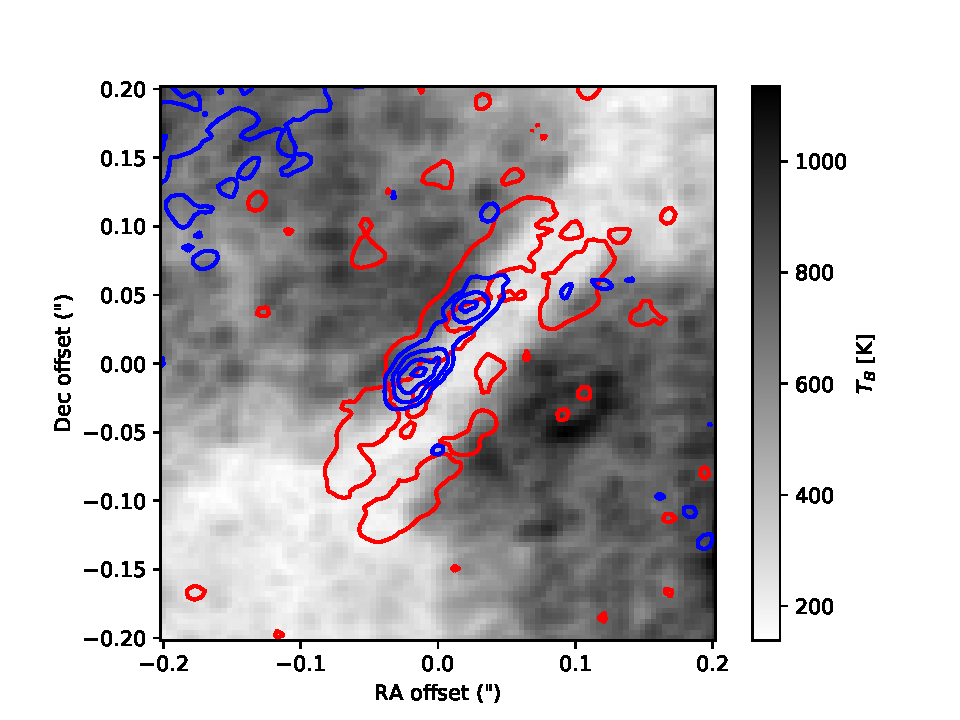
\includegraphics[scale=1,width=4in]{figures/SiO_8-7_on_NaClv=2_26-25.pdf}
\caption{Peak intensity map of SiO v=0 J=8-7 (gray scale), NaCl v=2 J=26-25
(red contour; 200 K) and {SiO v=5 J=8-7} (blue contours; 300, 400, 500, and 600
K).  The blue contours in the upper-left come from a blend with a different
line.
}
\label{fig:sioonnacl}
\end{figure*}


While the most prominent spectral features were the SiO and \water lines that
have previously been observed \cite{Goddi2013a,Hirota2014a}, there were dozens
of lines that remained unidentified in our initial study \cite{Ginsburg2018b}.
We have now identified these lines as transitions of NaCl and KCl, noting the
excellent correspondence between the observed and measured/catalogued
frequencies \cite{Caris2002a,Caris2004a,Muller2005a,Lovas2005b,Pickett1998a}.
We additionally searched databases of transitions of these same species with
more quanta of vibrational excitation, and found additional matches
\cite{Barton2014a,Cabezas2016a}, with confident detections up to as much as
$v=6$.

%AG: the v=7 detections are <5-sigma; they're probably real, but not confident.

The detection of highly vibrationally excited transitions of these species,
with upper-state energy levels of as much as $\sim$3000~K, is suggestive of
extreme physical or radiative conditions.  The emission from these lines comes
from a narrow range in both position and velocity.  By fitting thin Keplerian
disk models to the position-velocity diagrams of the lines, we constrain the
emission region to be 30-60 AU from the central source.  The observed emission
peaks at $\pm13$ AU above and below the midplane of the continuum disk, which
may be either a physical height or an effect of obscuration by the optically
thick continuum.  The emission does not extend beyond this height, indicating
that, unlike SiO and \water, the salts do not trace the outflow.

%BAM: We aren't allowed to tell the reader how to feel (in Science).  Meaning,
%we can't say something is 'surprising.'  That's up to the reader to decide.
%no "we were shocked to see shocks"?  Boo.

Once in the gas phase, however, we expect salts to rapidly deplete back into
dust grains \cite{Cherchneff2012a}.  Since we observe them in emission, with
narrow velocity line profiles, they must be released into the gas phase by
either grain destruction, or produced chemically from simple gas-phase
precursors, likely elemental atomic gas (either neutral or ionized Na and K).
Because previous studies have ruled out the presence of any atomic
recombination lines (from atomic ions recombining with electrons) in this
source, and therefore demonstrated that there is no ionized gas around Source I
\cite{Plambeck2016a,Baez-Rubio2018a}, we reject the atomic formation route. We
therefore suggest that the salts are produced by dust destruction, either
via sputtering by high-energy particles \cite{Schilke1997a} or by thermal
desorption of the outer dust layers \cite{Decin2016a}.  The small scale
height of the observed salt emission therefore implies that grain destruction
is an efficient and rapid process in disk-launched winds.

%Again, we can present our viewpoint based on the data, but it's up to the
%reader to decide if that is what 'must' be happening.

The vibrationally excited transitions observed suggest that radiative
excitation is important in this environment.  The molecular transitions we
observe have high Einstein A values, in the range $\sim10^{-3}-10^0$, and
correspondingly high critical densities $n_{cr} \sim10^{8}$ \percc for v=0 and
$n_{cr} \sim 10^{12}$ for $v>=1$, where $v$ is the vibrational quantum number.
Collisional excitation alone cannot explain the different vibrational states
being observed at a similar brightness level. The rovibrational $\Delta v=1$
transitions of NaCl and KCl occur in the 25-35 \um and 35-45 \um range,
respectively.  Since a blackbody with $T\sim100$ K peaks at $\lambda\sim30$
\um, and the observed disk brightness temperature is around 100-300 K at the
radii where salts are observed, it is plausible that strong radiation from the
disk in the mid-infrared is responsible for exciting the molecules.  However,
we have not been able to assemble a self-consistent model explaining both the
rotational and vibrational excitation ladders of NaCl or KCl.  In the
supplemental material, we describe  and evaluate several possible
excitation mechanisms that are less likely but not ruled out.

\begin{figure}
    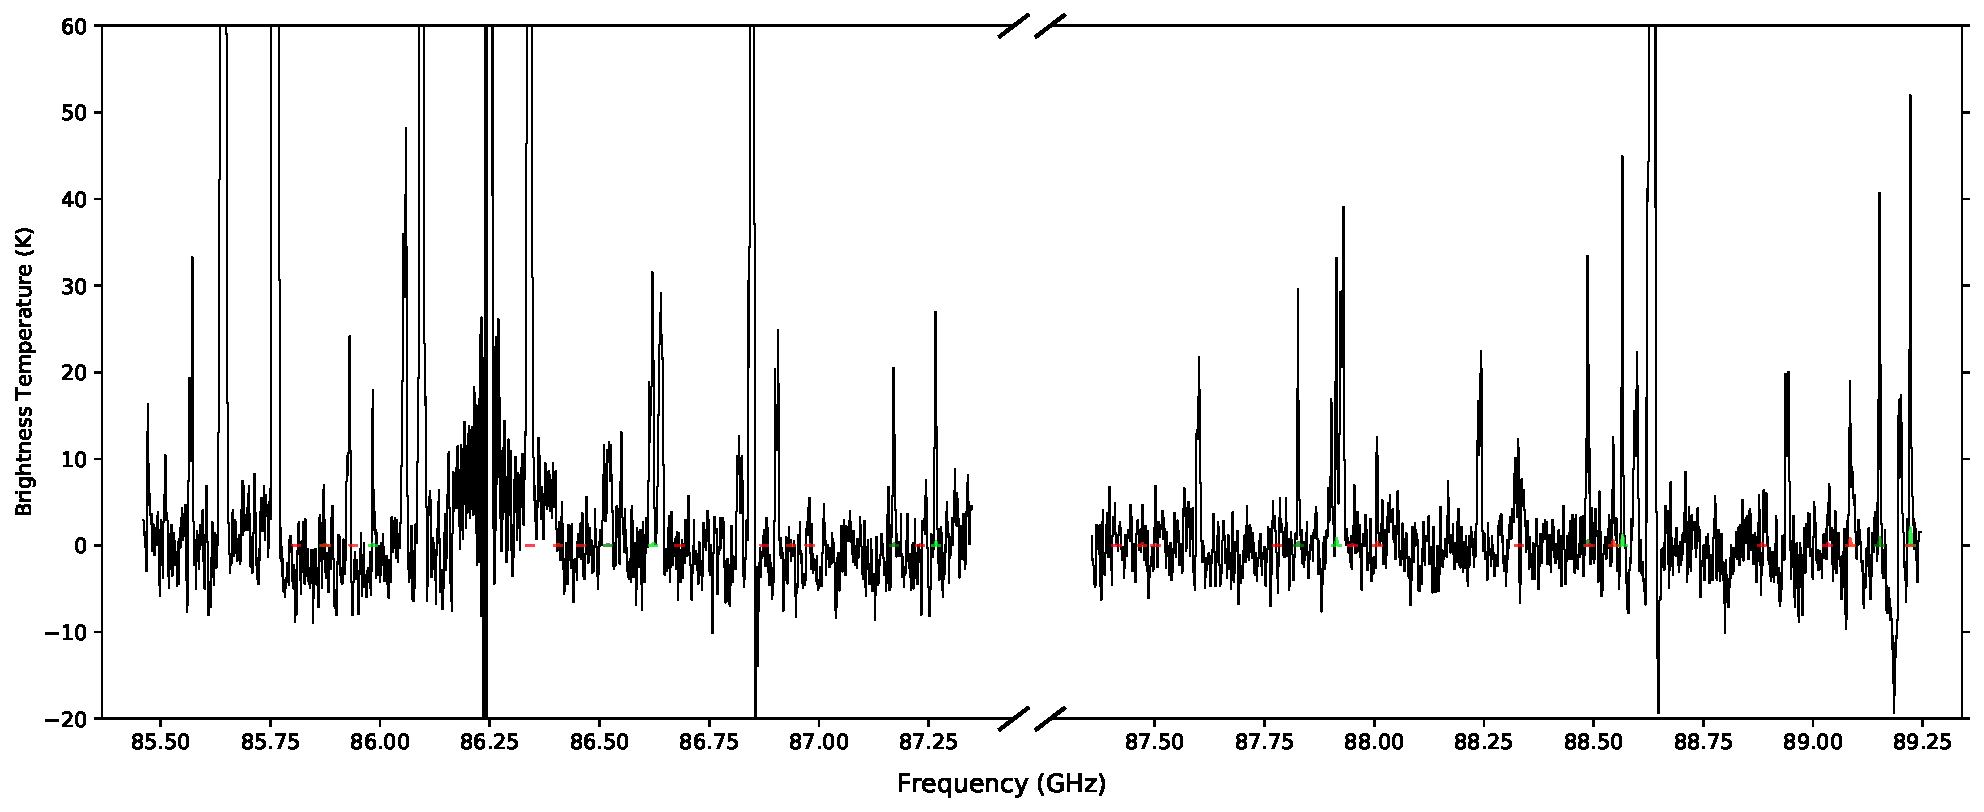
\includegraphics[scale=1,width=3.0in]{{figures/squash_lte_overlay_K_a_OrionSourceI_B3_spw1_robust0.5}.pdf}
    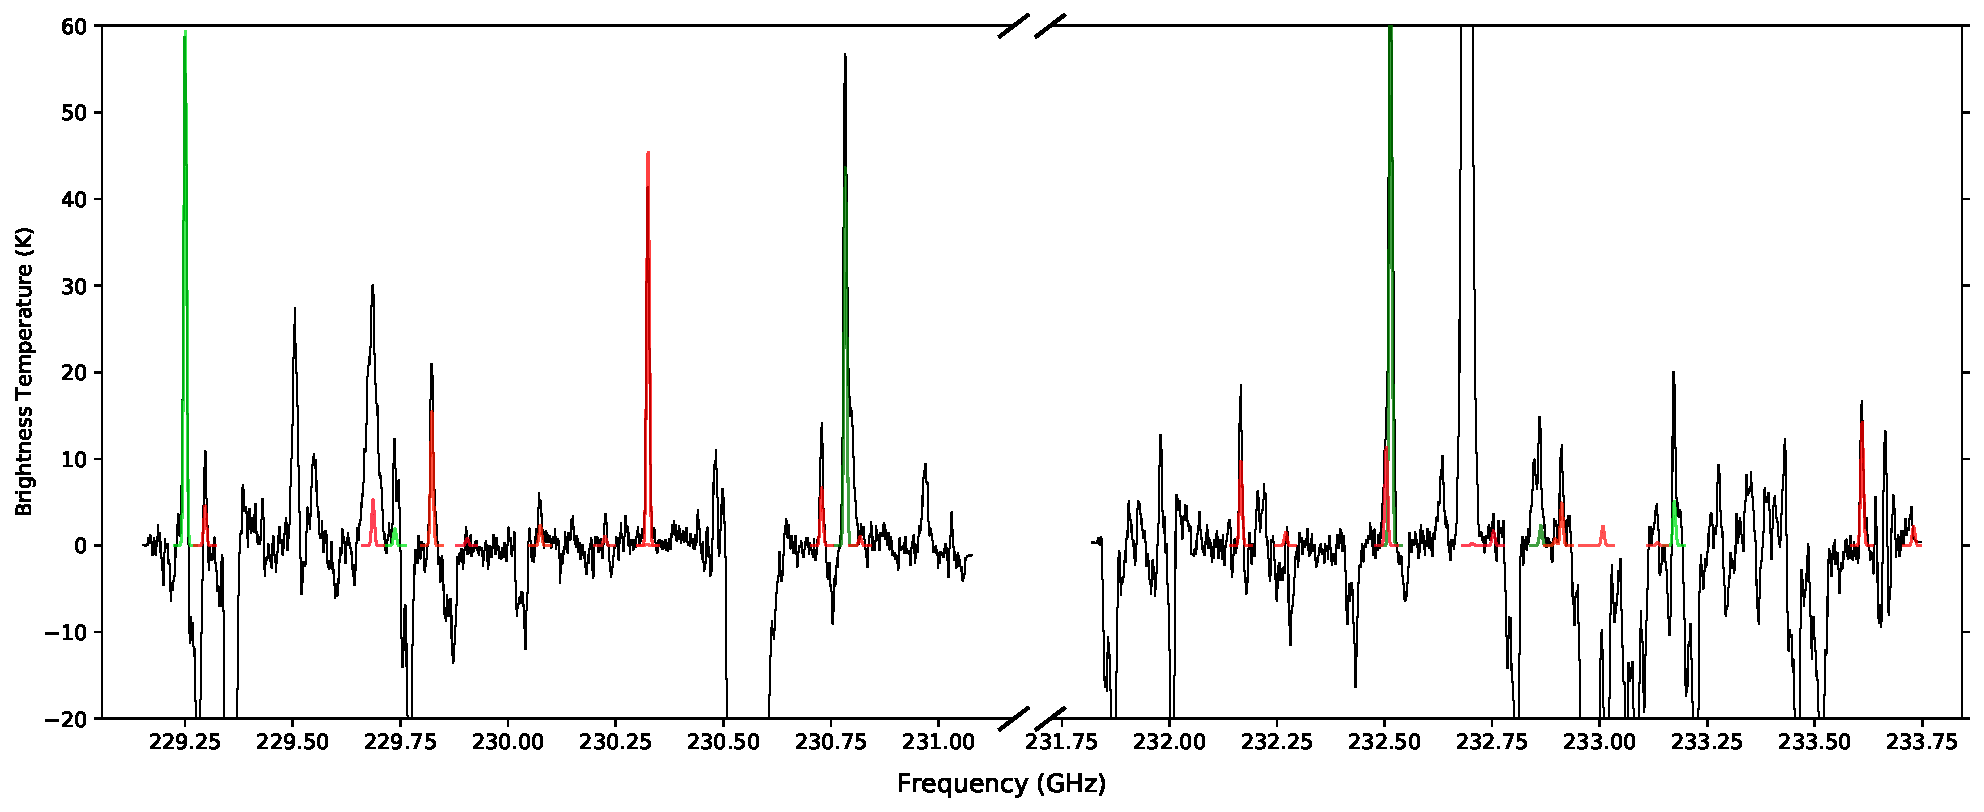
\includegraphics[scale=1,width=3.0in]{{figures/squash_lte_overlay_K_a_OrionSourceI_B6_spw1_robust0.5}.pdf}
    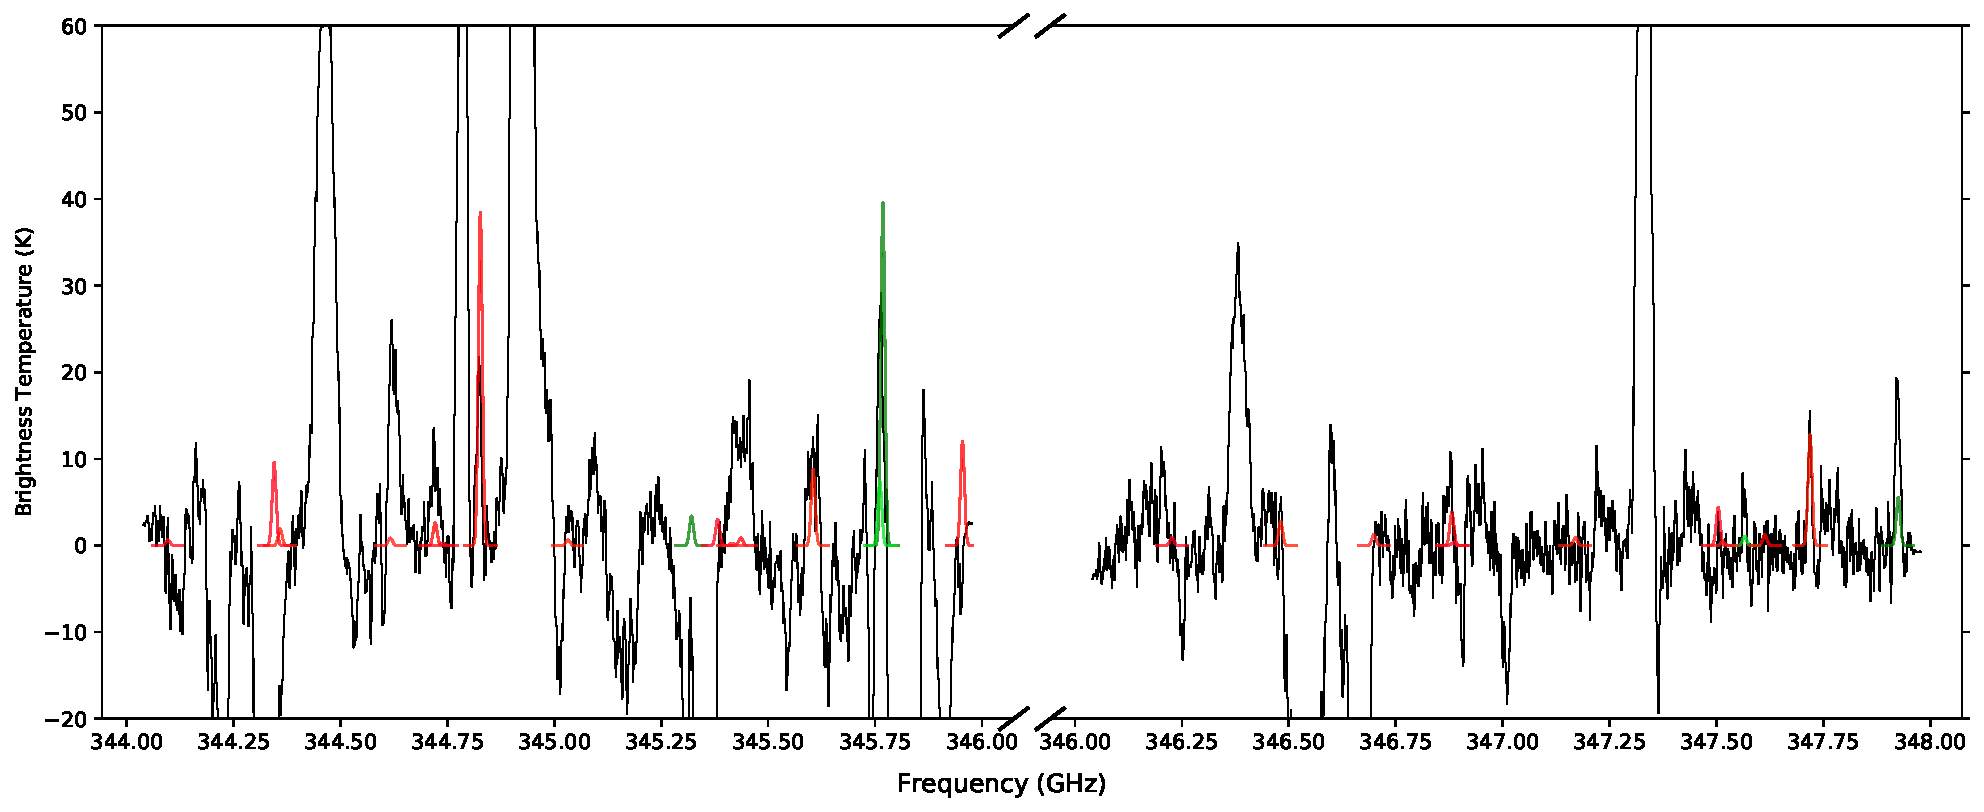
\includegraphics[scale=1,width=3.0in]{{figures/squash_lte_overlay_K_a_OrionSourceI_B7.lb_spw1_robust0.5}.pdf}
    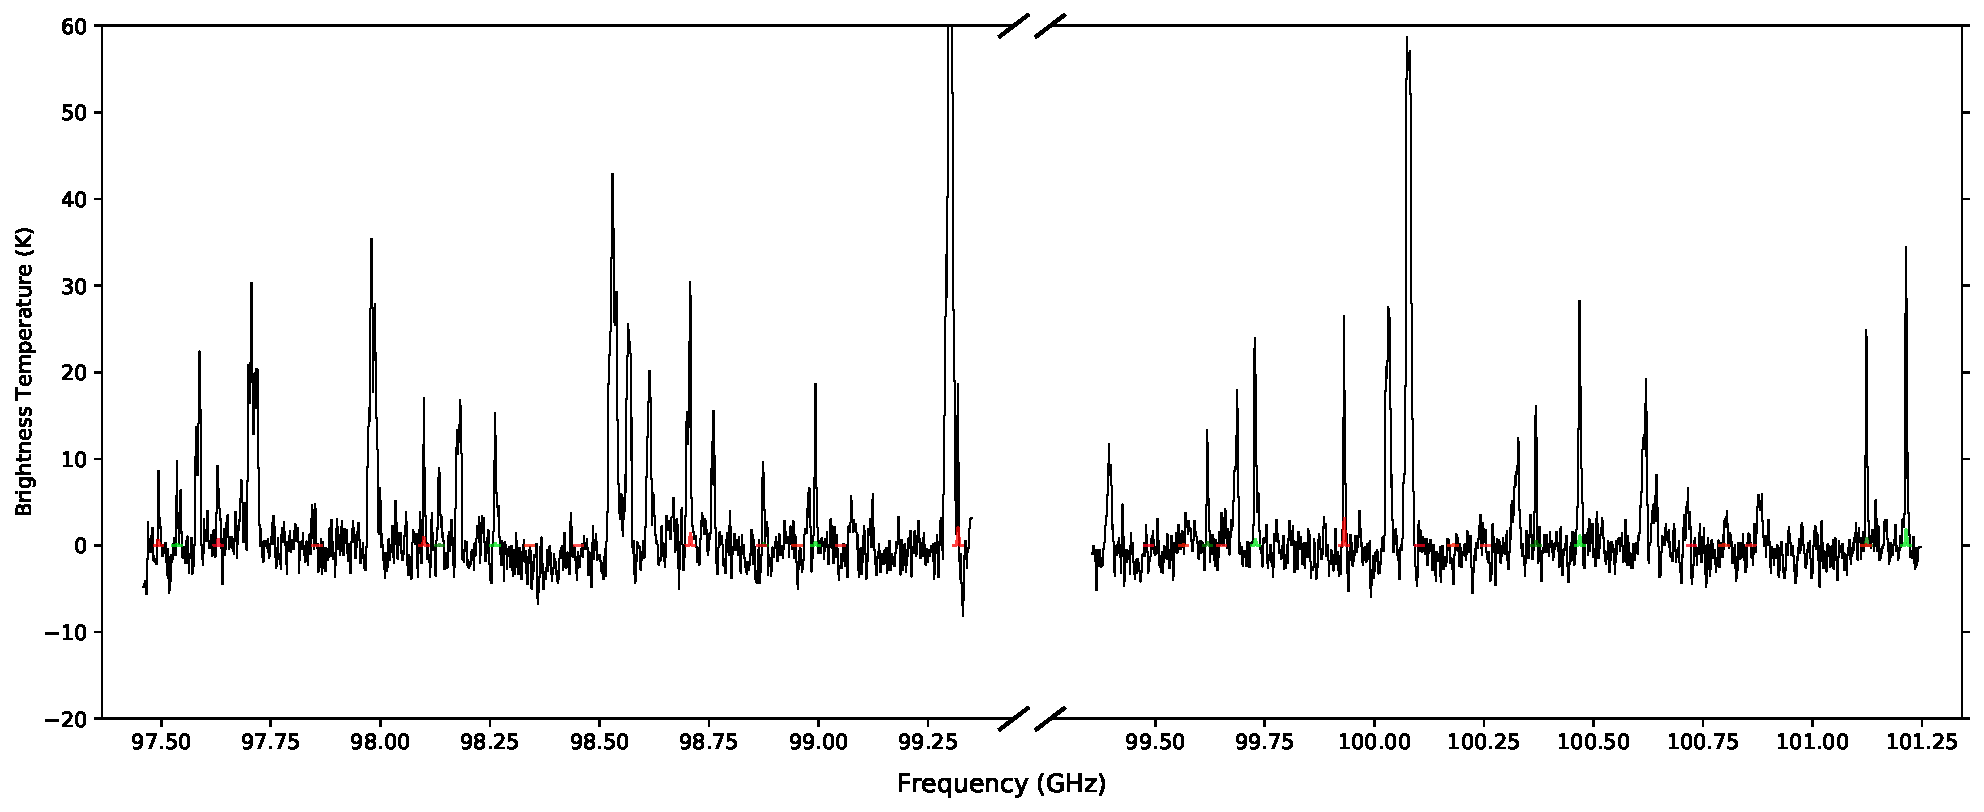
\includegraphics[scale=1,width=3.0in]{{figures/squash_lte_overlay_K_b_OrionSourceI_B3_spw3_robust0.5}.pdf}
    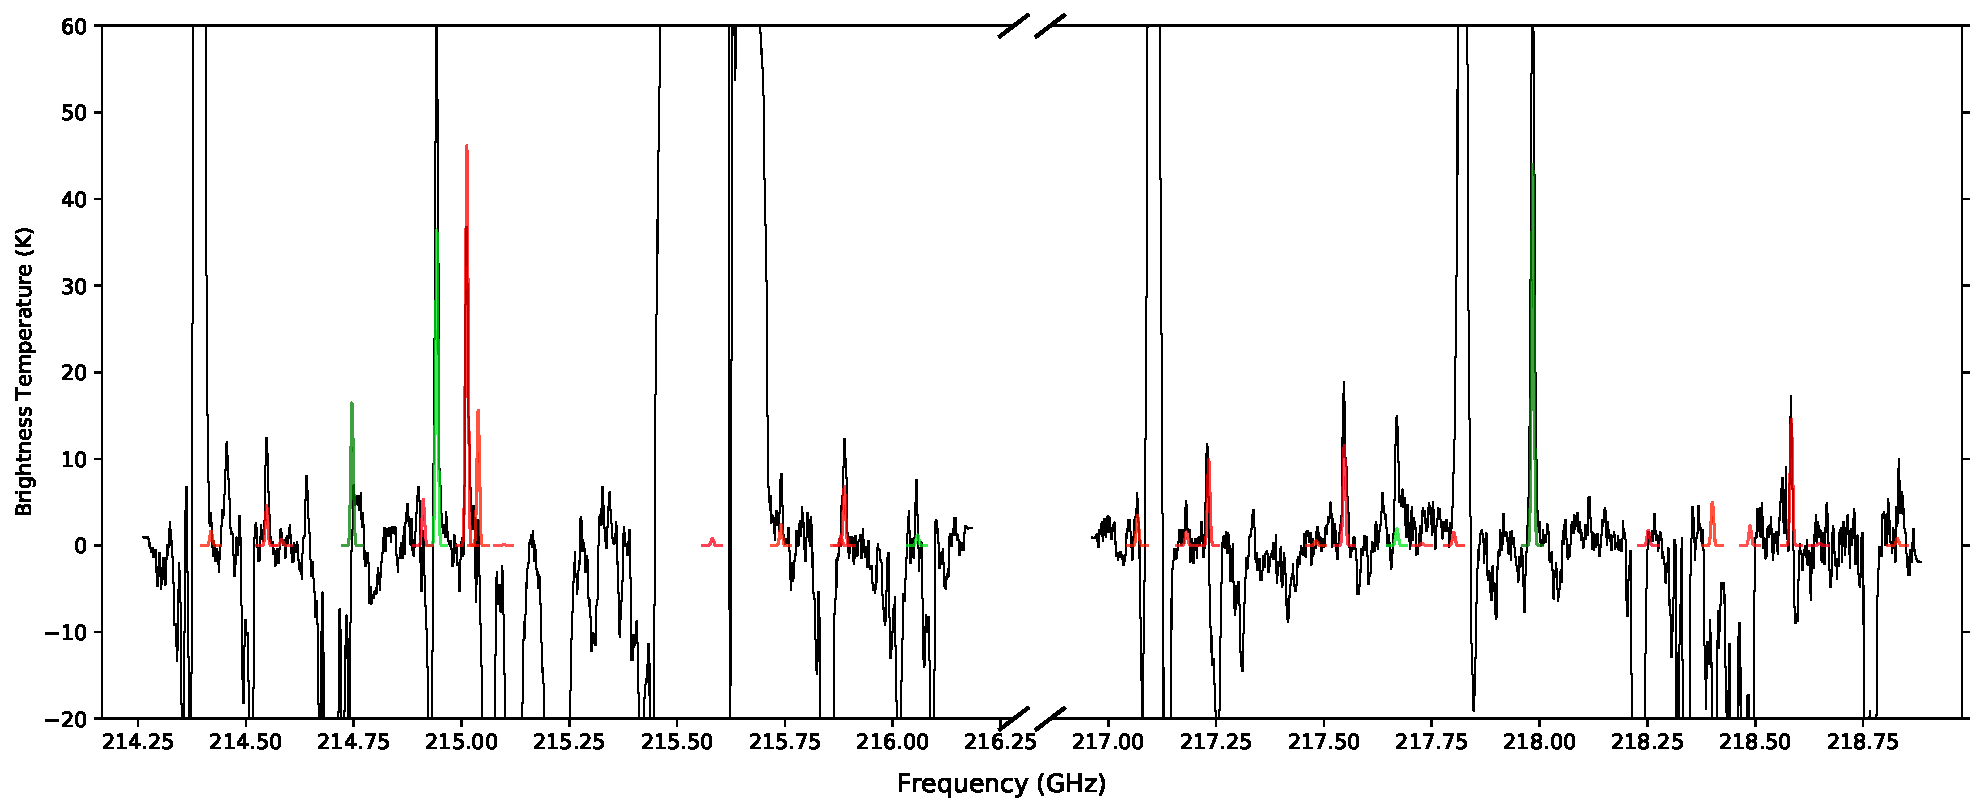
\includegraphics[scale=1,width=3.0in]{{figures/squash_lte_overlay_K_b_OrionSourceI_B6_spw3_robust0.5}.pdf}
    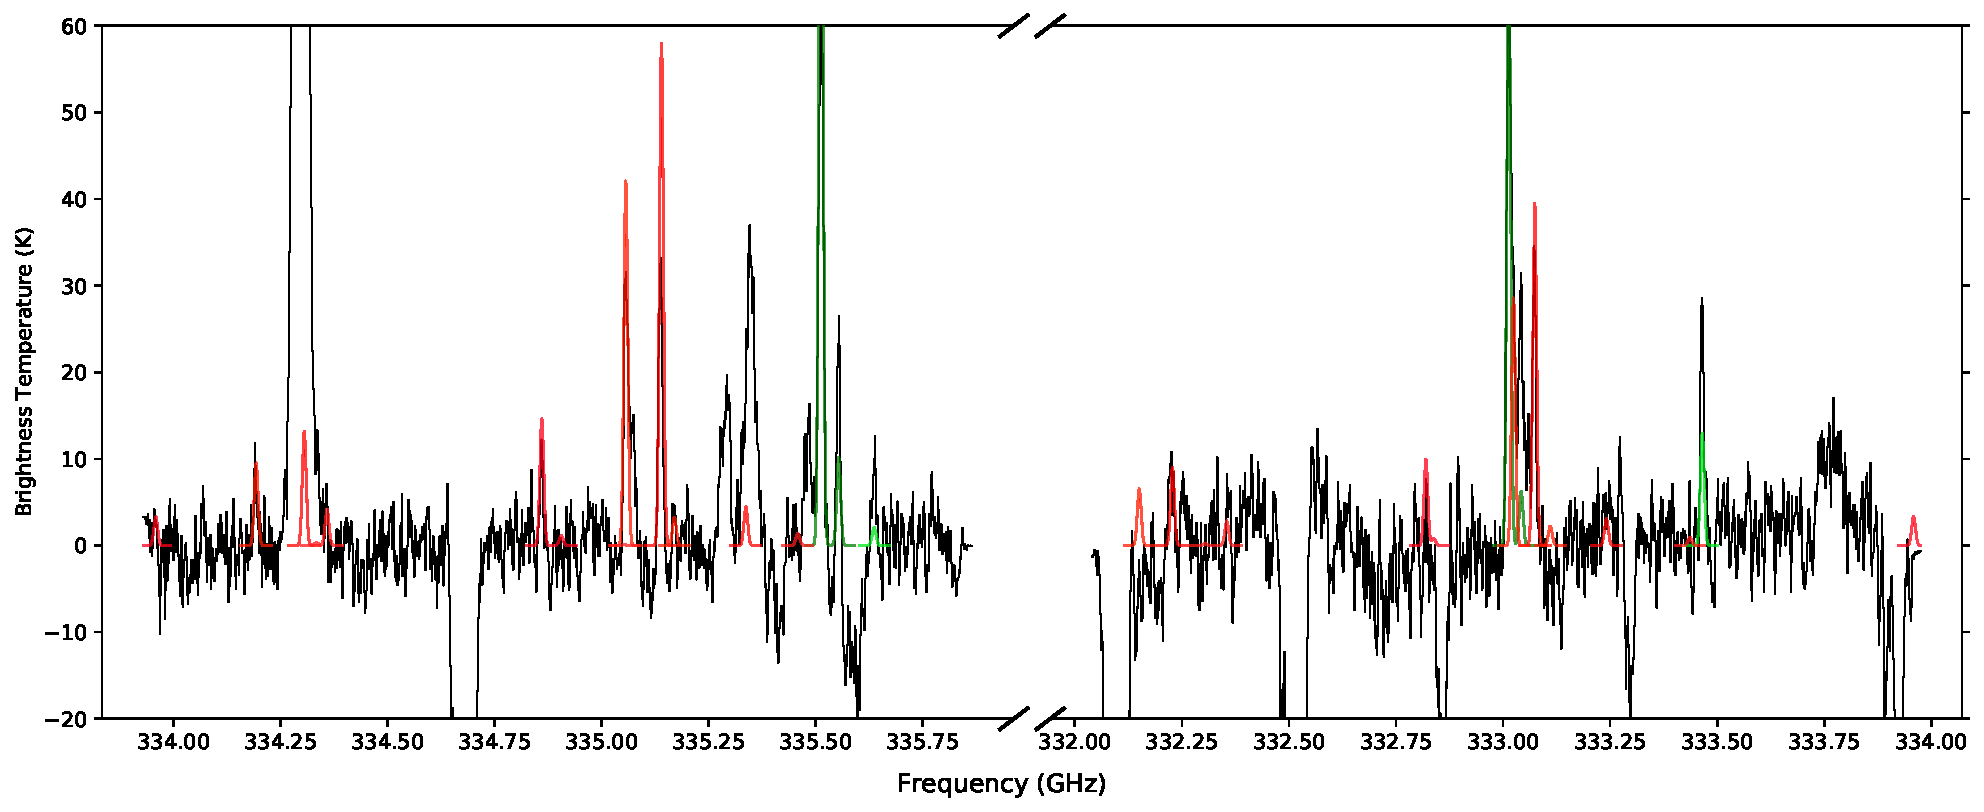
\includegraphics[scale=1,width=3.0in]{{figures/squash_lte_overlay_K_b_OrionSourceI_B7.lb_spw3_robust0.5}.pdf}
    \label{fig:spectra}
    \caption{Spectra with NaCl (green) and KCl (red) models overlaid}
\end{figure}


% The detection of NaCl and KCl in our current dataset was serendipitous.  As a
% result, the observations were not optimized for unraveling the physical and
% chemical conditions underlying their presence and excitation, hindering our
% ability to obtain a full picture of the exact utility of these salts as
% tracers.  Nevertheless, we obtain several important conclusions from these
% detections.

We conclude that these newly detected transitions uniquely trace the disk
around a massive protostar.  Since they appear to be an unambiguous tracer of
high-mass protostellar disks, if they behave the same in other high-mass disks,
they will facilitate kinematic measurements of disks and therefore direct mass
measurements of the contained stars.  Access to such a tool would finally make
direct comparisons between high- and low-mass star formation possible.

Since these molecules contain atoms usually trapped in dust and therefore
rarely seen in the molecular ISM, they may serve as a tool for directly
measuring absolute metallicity in an environment that is typically far too
chemically complex and obscured for other methods to work.  Since these
species are released into the ISM only by supernovae, these transitions
could prove a powerful probe of supernova feedback in high-extinction
regions. % this is pretty far-fetched...

% Of these species,
% Na is produced only in massive star supernovae, while K and Cl are produced in
% white dwarf supernovae  <-- I don't know if this is true.  cosmic-origins.org +
% wikipedia say so, but those are loose.  Arnett '96 doesn't seem to have a table
% of "this comes from here".

%This last paragraph should probably be two or three instead of one?  Note that
%we explicitly cannot include any 'forward-looking' projects that *we plan*
%(meaning, we cannot say that follow-up studies will look at X or Y).  We can
%speculate a bit (it's a fine line) on what these lines might be useful for in
%a general sense, however.

\bibliographystyle{Science}
\bibliography{extracted}

\end{document} 

